\documentclass[aps,preprint,groupedaddress,letterpaper]{revtex4-1}
%\documentclass[aps,twocolumn,groupedaddress]{revtex4-1}
\usepackage{graphicx,bm,hyperref,amsmath,amssymb}
\usepackage{natbib} % necessary for bibtex
\usepackage{float}
\usepackage{caption}
\usepackage{subcaption}
\begin{document}

\title{Fractal Dimension of the Diffusion Limited Aggregation Model on and off Lattice}

\author{Jacky Lin}
\affiliation{Department of Physics \& Astronomy, Bucknell University, 
Lewisburg, PA 17837}

%%%% Make sure that \maketitle command is after the abstract
\maketitle

\section{Abstract}
We study with computer simulations the fractal dimension, $d_f$, of the diffusion-limited aggregation model on-lattice as well as off-lattice. We vary stickiness which refers to the probability that the random walker would stick to the cluster, neighboring range, which refers to the range that determines whether a random walker is near a cluster, and random walk step size, $\alpha$. We measure and compare the fractal dimension of clusters under these circumstances. We determine $d_f$ as function of the number of particles in the cluster, and find that the cluster size at the end of simulation with 3000 particles is in the leveled off region, where the fractal dimension is close to the expected value of 1.71. By measuring the on-lattice fractal dimension of clusters with different stickiness and neighboring range separately, we find that with the increasing of stickiness and neighboring range, the fractal dimension decreases. In the off-lattice simulation, we find that the measured fractal dimension does not change with $\alpha$. Thus, we conclude that the fractal dimension is not always equal to the accepted on-lattice value of 1.71. 

\section{Introduction}
There are a variety of complicated patterns in nature. An enormous amount of these patterns is reproducible by modelling with fractal growth model. Fractal growth processes are a class of phenomena which produce self‐similar, disordered objects in the course of development far from equilibrium \cite{Sander2011}. For example, 
the Eden model describes the growth of some types of clusters, such as bacterial colonies and deposition of materials, grow by random accumulation of material on their boundary; 
the William and Bjerknes Model is a model for tumour in the basal layer of an epithelium \cite{WILLIAMS1972}; 
and the Ballistic aggregation models allow for overhangs on the surface as a result of allowing particles to attach themselves to the aggregate if a neighboring lattice point is occupied \cite{Pelliccione2008}.
Among them, diffusion-limited aggregation (DLA) is an idealized model describing the process by which matters irreversibly combine into dust, dendrites, and other fractal objects in the case where the rate-limiting step is a diffusion of matter to aggregate \cite{PhysRevB.27.5686}. In the DLA model, particles undergo a random walk (diffusion-limited) until they reach the cluster. DLA can be observed in many systems such as electrode position \cite{PhysRevLett.61.2558}, hele-Shaw flow \cite{PhysRevA.33.2663}, and dielectric breakdown \cite{doi:10.1143/JPSJ.55.2479}. One of the primary methods to study the DLA model is to use computer simulation.
 
The initial model of diffusion-limited aggregation was proposed by Witten and Sander in 1983 \cite{PhysRevB.27.5686}. Studies following this fundamental paper can be categorized into several ways. Some papers present simulation on certain particles or substances using this model, such as Baki and Badr’s Electroless, diffusion-limited aggregation of lead dendrites \cite{BAKI2021110586}. In other papers, the focus is on the simulation of the diffusion-limited aggregation model on different surfaces. For example, Choi, Crowdy, and Bazant applied this model on curved surfaces \cite{Choi}, and Eldan simulate DLA model on hyperbolic planes \cite{Eldan}. Another direction is to study the DLA model in multi-dimensions. Witten and Sander stated that DLA has no upper critical dimensions \cite{PhysRevB.27.5686}. Sander, Cheng, and Richter used this model in three dimensions \cite{dla3d}. Another way is investigating some scaling characteristics of the model, such as I.R. Nogueira, S.G. Alves, S.C. Ferreira explore the Scaling laws in the diffusion-limited aggregation of persistent random walkers \cite{scalelaw}, F.L. Braga, M.S. Ribeiro optimize algorithm for the simulation of the DLA \cite{2011CoPhC.182.1602B}.

% In this paper, we will further explore these features that occurs in the diffusion-limited aggregation model based on computer simulation. The primary job of this paper focuses on changing parameters involving in the simulation program of the DLA model to produce different features of the DLA model under these circumstances.

\section{Model}
Although such a model is applicable to multiple dimensions, we describe below the basic steps of Diffusion-Limited Aggregation model in two-dimensions. 

\subsection{On-Lattice Rules}

First set of rules is for on-lattice simulation of DLA model, and it is described in Witten and Sander’s paper \cite{PhysRevB.27.5686}.

\begin{enumerate}
    \item Initially, the 2D lattice $L$ is initialized with a cluster containing one particle in the center of the lattice.
    \item Launch a random particle at a circle of radius $r_{\rm launch}$ larger than the largest distance from the seed of a particle belonging to the cluster $r_{\rm launch} \gg r_{\rm aggr}+ 2$.
    \item Undergo a random walk with each step being UP, DOWN, LEFT, RIGhT with equal probability \cite{doi:10.1063} (See Fig.~\ref{random_walk}).
    
    \begin{figure}[h]
    \centering
    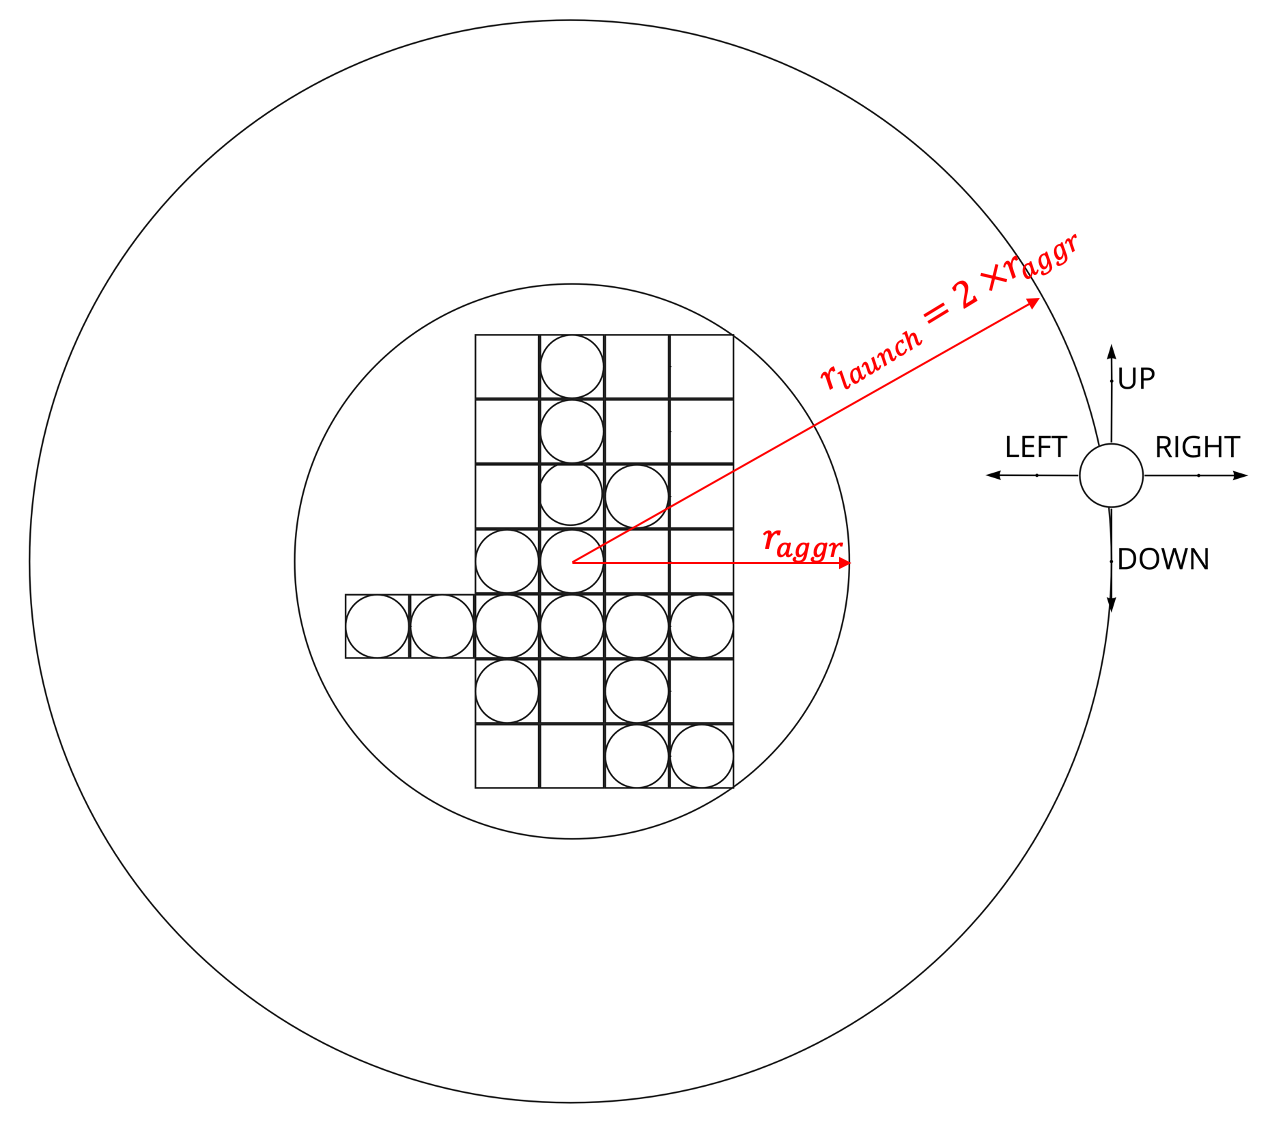
\includegraphics[width=4.0in]{img/RandomWalk.png}
    \caption{Random Walk in Diffusion-Limited Aggregation
    \label{random_walk}}
    \end{figure}
    
    \item The trajectory is stopped whenever the condition is met:
    \begin{enumerate}
        \item The random walk particle sticks to the cluster when it arrives at a perimeter site of the cluster (The UP, DOWN, LEFT, RIGhT site of random walker is nearest neighbor of site which already belongs to cluster) 
        \item The random walk particle is beyond a circle that has 2 times the aggregation size:
        \begin{equation}
            r_{\rm max} = r_{\rm aggr} \times 2
        \end{equation}
    \end{enumerate}
    
    \item Steps 2 to 4 will be repeated until the total number of particles in the cluster reaches N particles. (See Fig.~\ref{basic_steps})
    
    \begin{figure}[h]
    \centering
    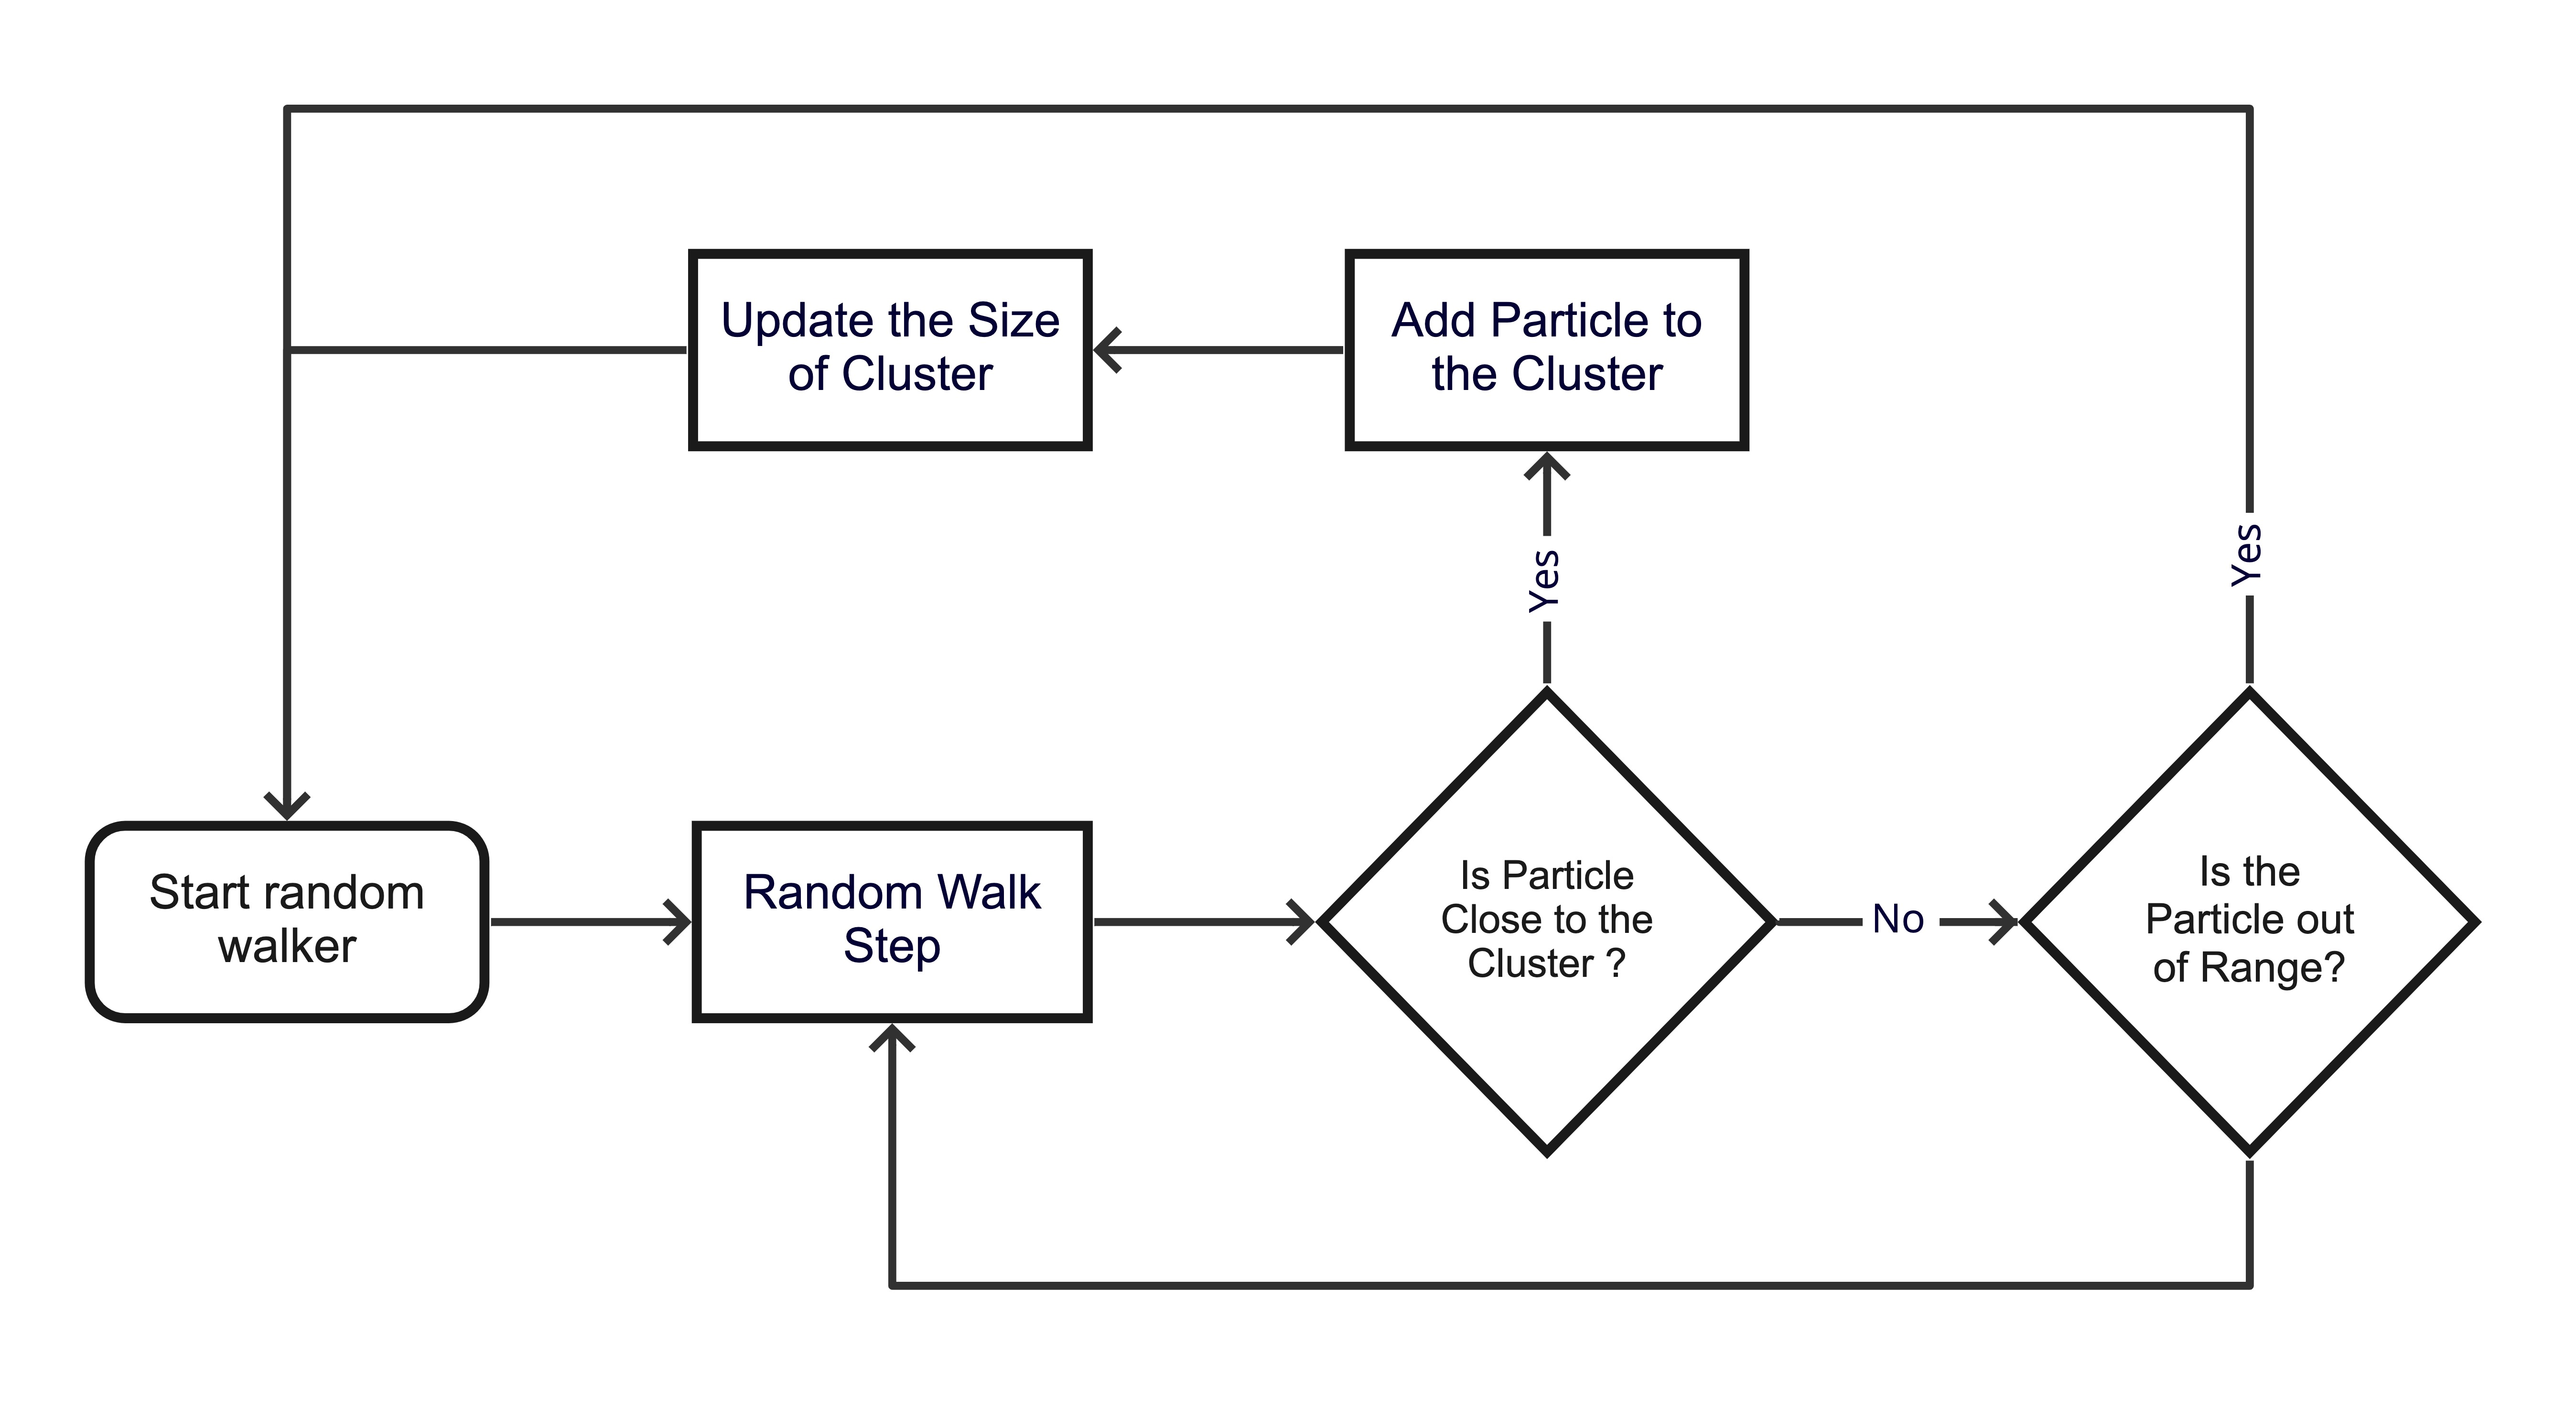
\includegraphics[width=4.0in]{img/BasicStep.jpg}
    \caption{Flowchart of Basic Steps in DLA Model 
    \label{basic_steps}}
    \end{figure}
\end{enumerate}

\subsection{Off-lattice Rules}

The second set of rules is for off-lattice simulation of DLA model \cite{scalelaw},

\begin{enumerate}
    \item Initially, there is a two dimensional space initialized with a cluster containing one particle of radius $r_{\rm p}$ on the center of this area.
    
    \item Launch a random particle with radius of $r_{\rm p}$ at a circle of radius greatly larger than the largest distance from the seed of a particle belonging to the cluster $r_{\rm launch}= r_{\rm p} \times (r_{\rm aggr}+2)$
    
    \item The particle undergoes a random walk, where the position of the $n$-th step is given by:
    
    \begin{equation} \label{off}
    \begin{split}
    x_n &=x_{n-1} + \alpha\cos{\phi_n} \\
    y_n &=y_{n-1} + \alpha\sin{\phi_n}
    \end{split}
    \end{equation}
    
    where the direction of the nth step depends on the preceding one as
    \begin{equation}
        \phi_n\ = \phi_{n-1}\ +\ \eta_n
    \end{equation}
    where $\eta_n$ is a random variable uniformly distributed in the interval $\left(-\delta_\theta/2,\delta_\theta/2\right)$ and the $\delta_\theta$ limits the next move direction inside an angular opening of size $0 \le \delta_\theta\le2\pi$, centered in the direction of the previous step. The initial value of $\phi_0$ is a random angle uniformly distributed $n$ the interval $(0,2\pi)$.
    
    \item The trajectory is stopped whenever the condition is met:
    \begin{enumerate}
        \item The particle visits a position adjacent to the cluster where it sticks, that is -- two particles $i$ and $k$ are neighbors if $|\vec{r}_i-\vec{r}_k| < 2 r_{\rm p}$, where particle $i$ is a member of cluster and $k$ is a random walker particle.
        \item The particle is discarded whenever it crosses a distance $r_{\rm launch}\gg 2\times r_{\rm p} \times r_{\rm aggr}$
    \end{enumerate}
    
    \item Steps 2 to 4 will be repeated until the total number of particles in cluster reaches N particles. All the particle in the cluster have a radius of $r_{\rm p}$
    
\end{enumerate}


\section{Result}
\subsection{On-Lattice Result}
\subsubsection{Fractal Dimension}
\begin{figure}[h]
\centering
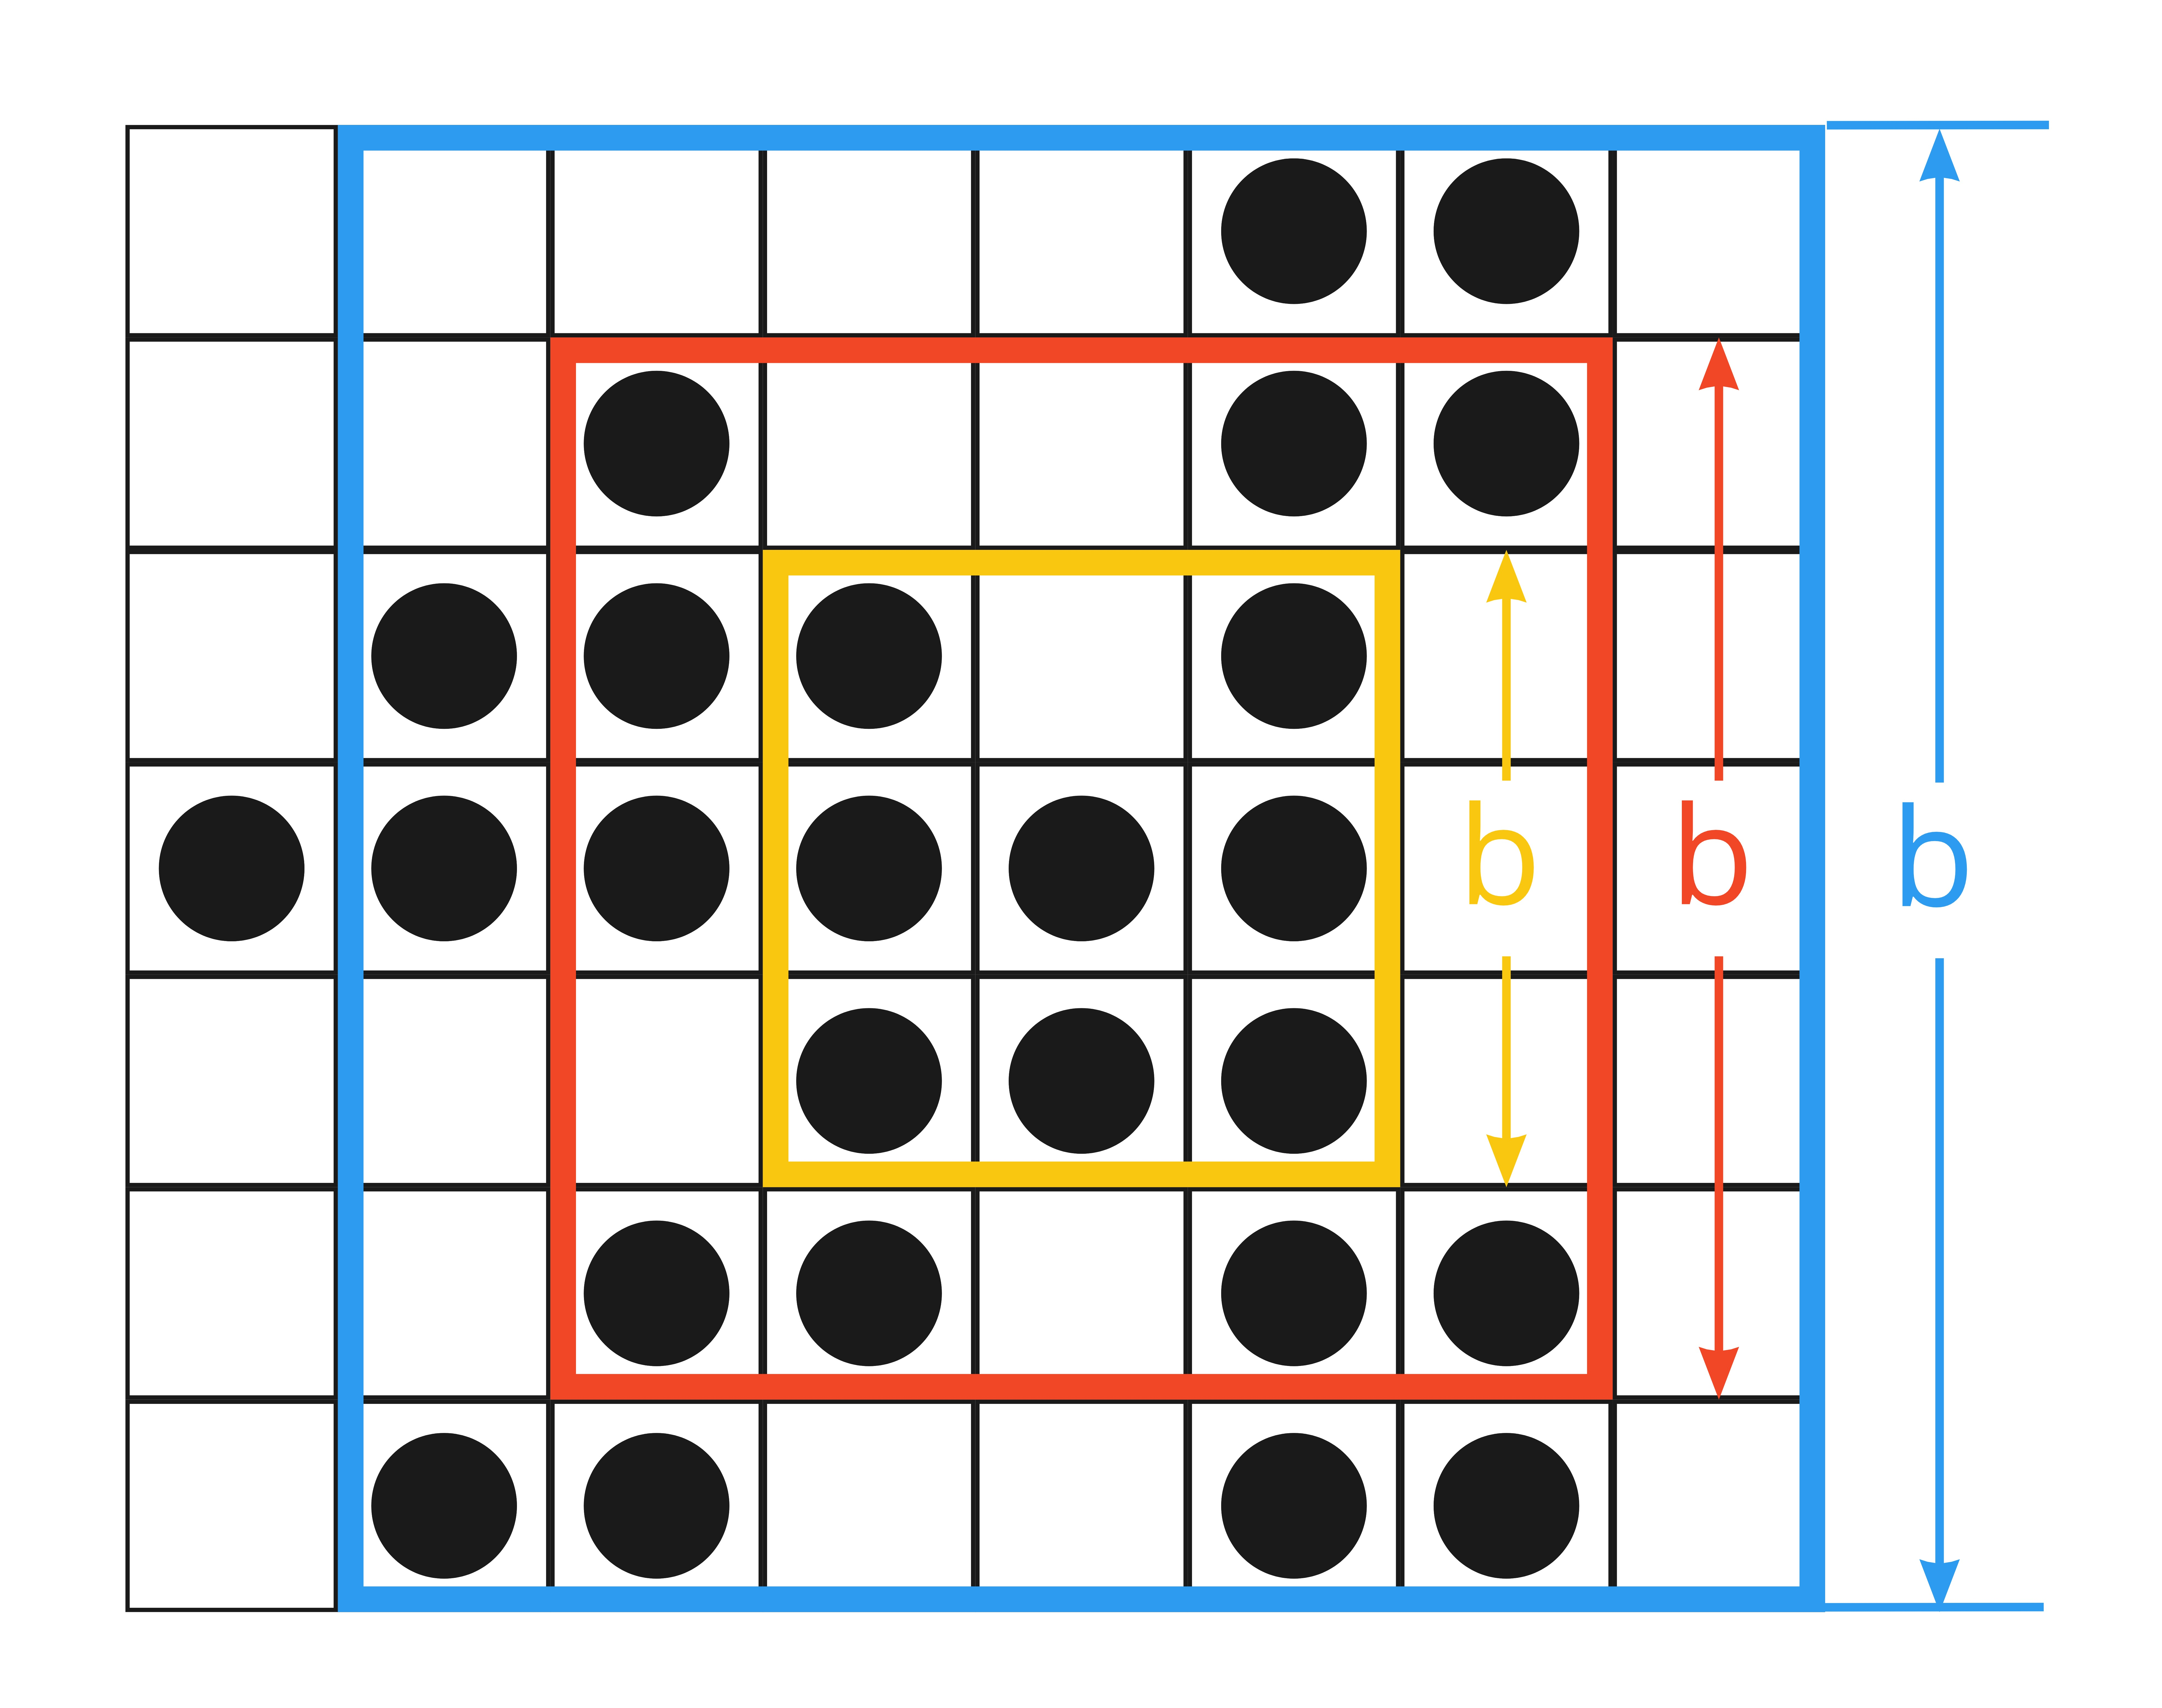
\includegraphics[width=4.0in]{img/bs.jpg}
\caption{Measurement of $b$ and $s$l 
\label{bs}}
\end{figure}

A fractal dimension quantifies how the mass or number of occupied sites, $N$, scales with the length, $b$, of the observed pattern
\begin{equation}
    N = c \times b ^{d_f}
\end{equation}
To get the fractal dimension $d_f$ we use the following relation.
\begin{equation}
\label{eqn:lndf}
    \ln(N) = \ln(c) + d_f \times \ln(b)
\end{equation}
(See Fig.~\ref{bs}) where $N$ is the number of occupied sites in a box of size $b \times b$ centered on the middle of the lattice, $c$ is some constant. $b$ is the length of square for which we count the number of occupied sites. For example, as shown in the above graph, the $b$ increases from 3 to 7 (yellow box to red box to blue box). 

To measure the fractal dimension for on-lattice final configurations, we measure the number of particles $N$ within a box of size $b$ as a function of $b$. Fig.~\ref{dfplot} shows the resulting $\ln(N)$ as a function of $\ln(b)$. When the size is small, the number of data points is sparse, while when the box size is large, the data points are dense. The density of data points increases as the size of the box increases.

\begin{figure}[h]
\centering
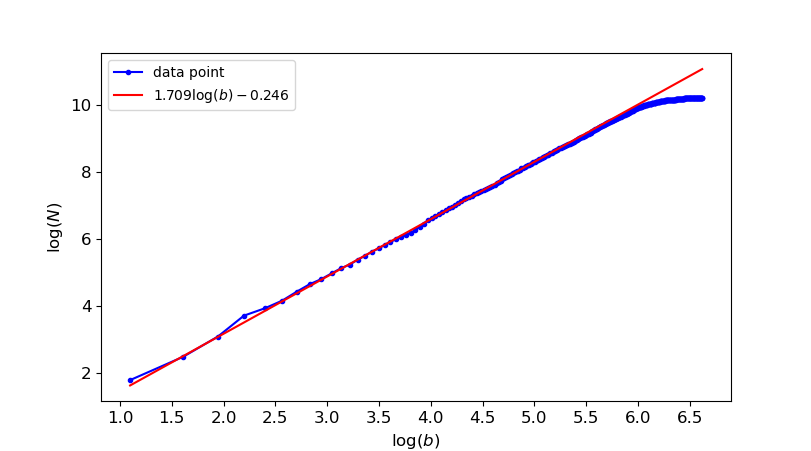
\includegraphics[width=5.0in]{img/dfplot.png}
\caption{Example of $\log(N)$ as a function of $\log(b)$ (Cluster Size = 27223)
\label{dfplot}}
\end{figure}

Included in Fig.~\ref{dfplot} is a linear fit of intercept -0.246 and slope 1.709. According to Eq.~\ref{eqn:lndf}, we have the fractal dimension of this cluster is $d_f = 1.709$

As expected, when the box size is larger than the distance from the furthest particle to the center, the size of the cluster, $N$, reaches a plateau. As a consequence, when applying the polynomial fitting to the data points, we choose the range avoiding sparse data points and flattening data points to obtain the fractal dimension of the cluster. 

\subsubsection{Cluster Size}

% Fig.~\ref{dfboxplot} shows the measured fractal dimension as a function of number of cluster particles at the end of the simulation run, $N_{\rm max}$, varying from 100 to 20000 particles. By comparing $N_{\rm max}$ and corresponding fractal dimension, we could observe a positive relationship between the number of particles in the cluster and the difference between the measured fractal dimension and theoretical fractal dimension of the DLA model. 

% \begin{figure}[h]
% \centering
% 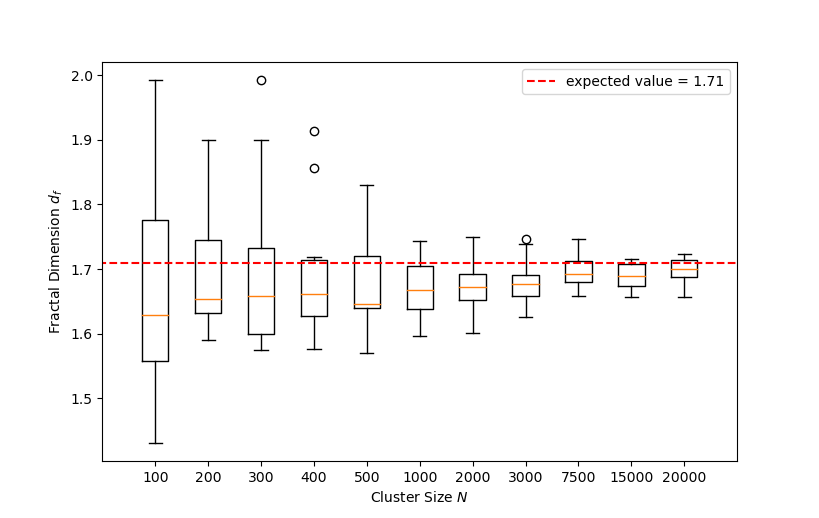
\includegraphics[width=5.0in]{img/PNum/box.png}
% \caption{Box plot of fractal dimension Final Cluster Size of 10 Independent Simulation Runs
% \label{dfboxplot}}
% \end{figure}

\begin{figure}[h]
     \centering
    %  \begin{subfigure}[h]{0.3\textwidth}
    %      \centering
    %      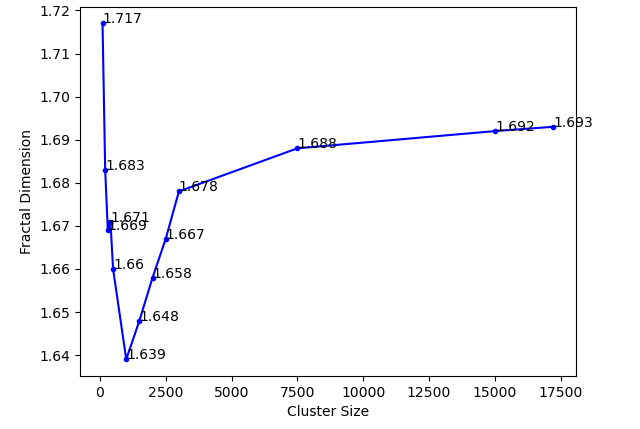
\includegraphics[width=\textwidth]{img/PNum/dfClusterSize.png}
    %      \caption{Fractal Dimension vs. Final Cluster Size For Single Simulation Runs}
    %      \label{dfcs}
    %  \end{subfigure}
    %  \hfill
     \begin{subfigure}[h]{0.45\textwidth}
         \centering
         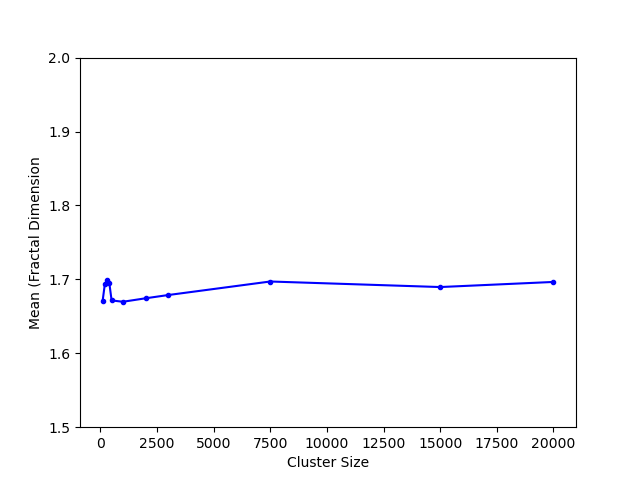
\includegraphics[width=\textwidth]{img/PNum/std.png}
         \caption{Mean Fractal Dimension vs. Final Cluster Size of 10 Independent Simulation Runs}
         \label{dfcsm}
     \end{subfigure}
     \hfill
     \begin{subfigure}[h]{0.45\textwidth}
         \centering
         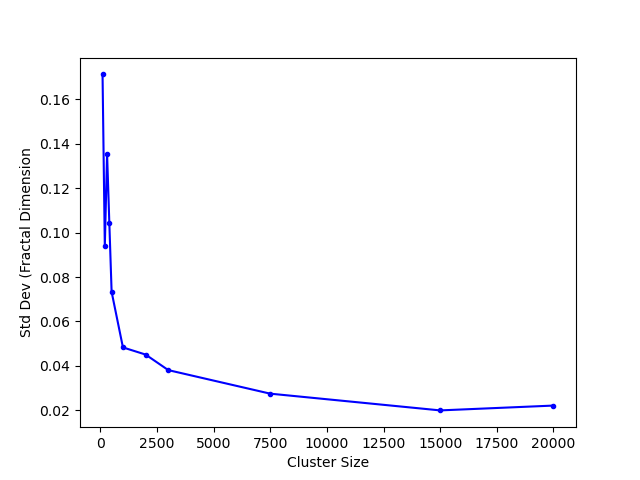
\includegraphics[width=\textwidth]{img/PNum/mean.png}
         \caption{Std Dev (Fractal Dimension) vs. Final Cluster Size of 10 Independent Simulation Runs}
         \label{dfcsstd}
     \end{subfigure}
\end{figure}




The first graph above (See Fig.~\ref{dfcsm}) plots mean fractal dimension with different final cluster size of 10 independent simulation runs. The second graph above (See Fig.~\ref{dfcsstd}) plots the standard deviation of measured fractal dimension with different final cluster size of 10 independent simulation runs. 

% When the cluster size at the end of simulation, $N_{\rm max}$, is larger than 3000, the measured fractal dimension is increased slightly with a large change of the $N_{\rm max}$. On the contrary, when $N_{\rm max}$ is small $( N_{\rm max} \leq 1000)$, the changes in measured fractal dimension largely decreased with small changes in the $N_{\rm max}$. When the $N_{\rm max}$ is between 1000 to 3000, the fractal dimension is largely increased with small changes in $N_{\rm max}$.Although the fractal dimension is large and closer to the standard fractal dimension of value 1.71 in the range 0 to 1000, the data size in this range is small, which means that a small change in one data point would cause the fractal dimension to vary significantly. This variation in data of small final size of cluster is also indicated
In plot of mean fractal dimension, mean fractal dimensions of 10 independent simulation runs across all final cluster size $N_{\rm max}$ do not fluctuated as the increase of cluster size. however, in the plots of standard deviation, We can see a drop in standard deviation of fractal dimension as the increases in the cluster size. Thus, even if the mean of fractal dimension for all cluster size is relatively the same, the smaller cluster size with high standard deviation is not reliable. For very large clusters, fractal dimension levels off, that means that we are no longer fighting finite size effects but that we reach a bulk value. Thus, we can observe that the cluster size at the end of simulation with 3000 particles is in the leveled off region, so the extra computational time is not needed.

\subsubsection{Stickiness}

\begin{figure}[h]
     \centering
     \begin{subfigure}[h]{0.23\textwidth}
         \centering
         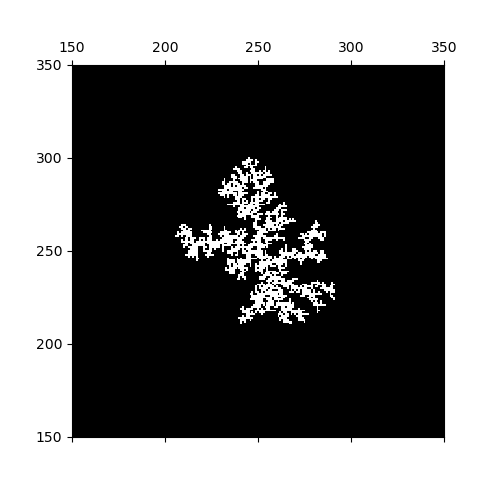
\includegraphics[width=\textwidth]{img/stickiness/st0.1.png}
         \caption{$\text{stickiness} = 1$}
         \label{st1}
     \end{subfigure}
     \hfill
     \begin{subfigure}[h]{0.23\textwidth}
         \centering
         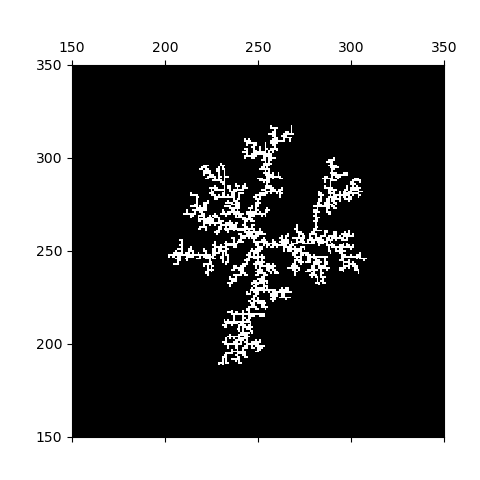
\includegraphics[width=\textwidth]{img/stickiness/st0.25.png}
         \caption{$\text{stickiness} = 0.25$}
         \label{st0.25}
     \end{subfigure}
     \hfill
     \begin{subfigure}[h]{0.23\textwidth}
         \centering
         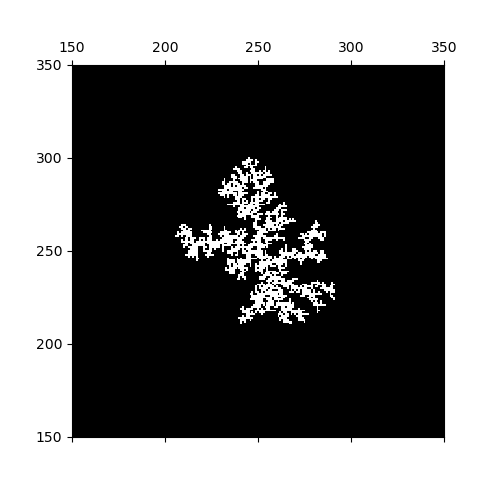
\includegraphics[width=\textwidth]{img/stickiness/st0.1.png}
         \caption{$\text{stickiness} = 0.1$}
         \label{st0.1}
     \end{subfigure}
     \hfill
     \begin{subfigure}[h]{0.23\textwidth}
         \centering
         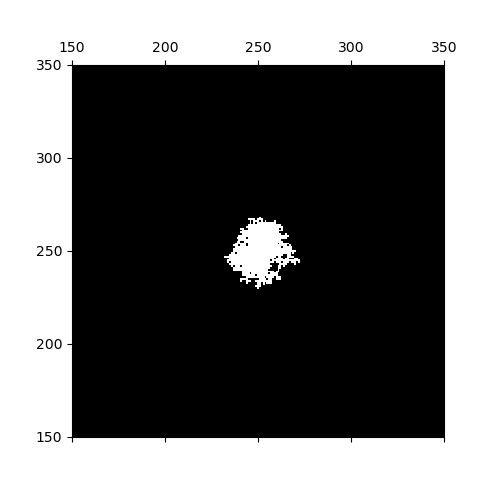
\includegraphics[width=\textwidth]{img/stickiness/st0.001.png}
         \caption{$\text{stickiness} = 0.01$}
         \label{st0.01}
     \end{subfigure}
        \caption{Clusters with Different Stickiness ($N = 3000$)}
        \label{sts}
\end{figure}

\begin{figure}[h]
\centering
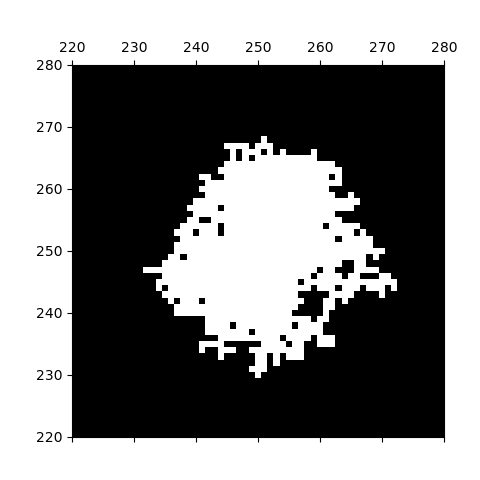
\includegraphics[width=3.0in]{img/stickiness/zoomin.png}
\caption{Cluster with Stickiness = 0.001 ($N = 3000$)
\label{stzoom}}
\end{figure}

Stickiness, $P_{\rm stick}$ refers to the probability that the random walker would stick to the cluster. By default, this value is set to 1. here we modify the stickiness by add a probability to Step 4a such that by certain probability the random walker is stick to cluster, and if the random walker isn't stick to cluster, it continues the random walk. By varying the stickiness, we could observe clusters with different densities. As shown in Fig.~\ref{sts}, for fixed $N$, the lower the stickiness the more condensed these clusters are. 

At stickiness equals 0.01, the cluster almost forms a circular disk. There are few empty spots remaining within the cluster (See Fig.~\ref{stzoom}).

\begin{figure}[h]
     \centering
     \begin{subfigure}[h]{0.45\textwidth}
         \centering
         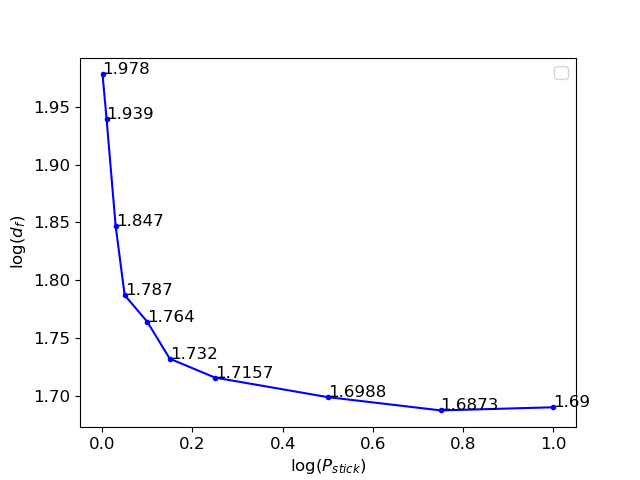
\includegraphics[width=\textwidth]{img/stickiness/dfst.png}
         \caption{Mean Fractal Dimension($N = 3000$)}
         \label{dfst}
     \end{subfigure}
     \hfill
     \begin{subfigure}[h]{0.45\textwidth}
         \centering
         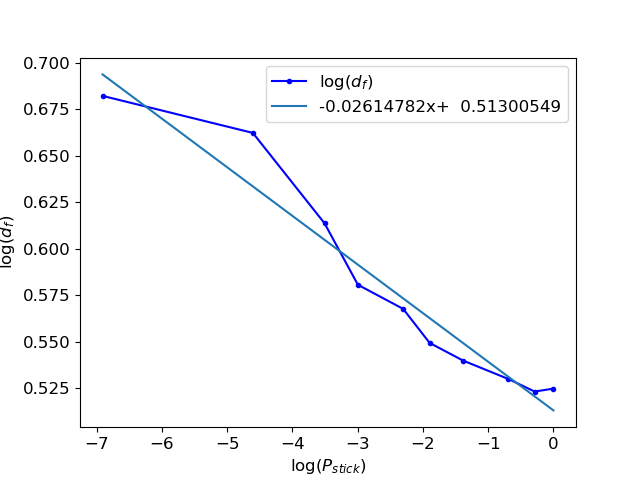
\includegraphics[width=\textwidth]{img/stickiness/logdfst.png}
         \caption{Log-log Plot of Mean Fractal Dimension}
         \label{logst}
     \end{subfigure}
        \caption{Fractal Dimension with Different Stickiness ($N = 3000$)}
        \label{sts}
\end{figure}

By measuring the fractal dimension of clusters with different stickiness, we could see that the lower the stickiness, the higher the fractal dimension (See Fig.~\ref{dfst}). Fig.~\ref{logst} shows a log-log plot of mean fractal dimension with respect to the stickiness, which indicates a inverse correlation between the increase in fractal dimension and decrease of stickiness. The max value is 1.978 when we set the stickiness to 0.01. In this case, the fractal dimension is near to 2. Since any 2-dimensional closed shapes have a fractal dimension of 2, we could conclude that as we decrease the stickiness of the cluster, the fractal dimension would infinitely approaching 2. This demonstrates that when we have stickiness infinitely approaching 0, the cluster would eventually form a 2-dimensional shape.

\subsubsection{Neighboring Range}

\begin{figure}[h]
\centering
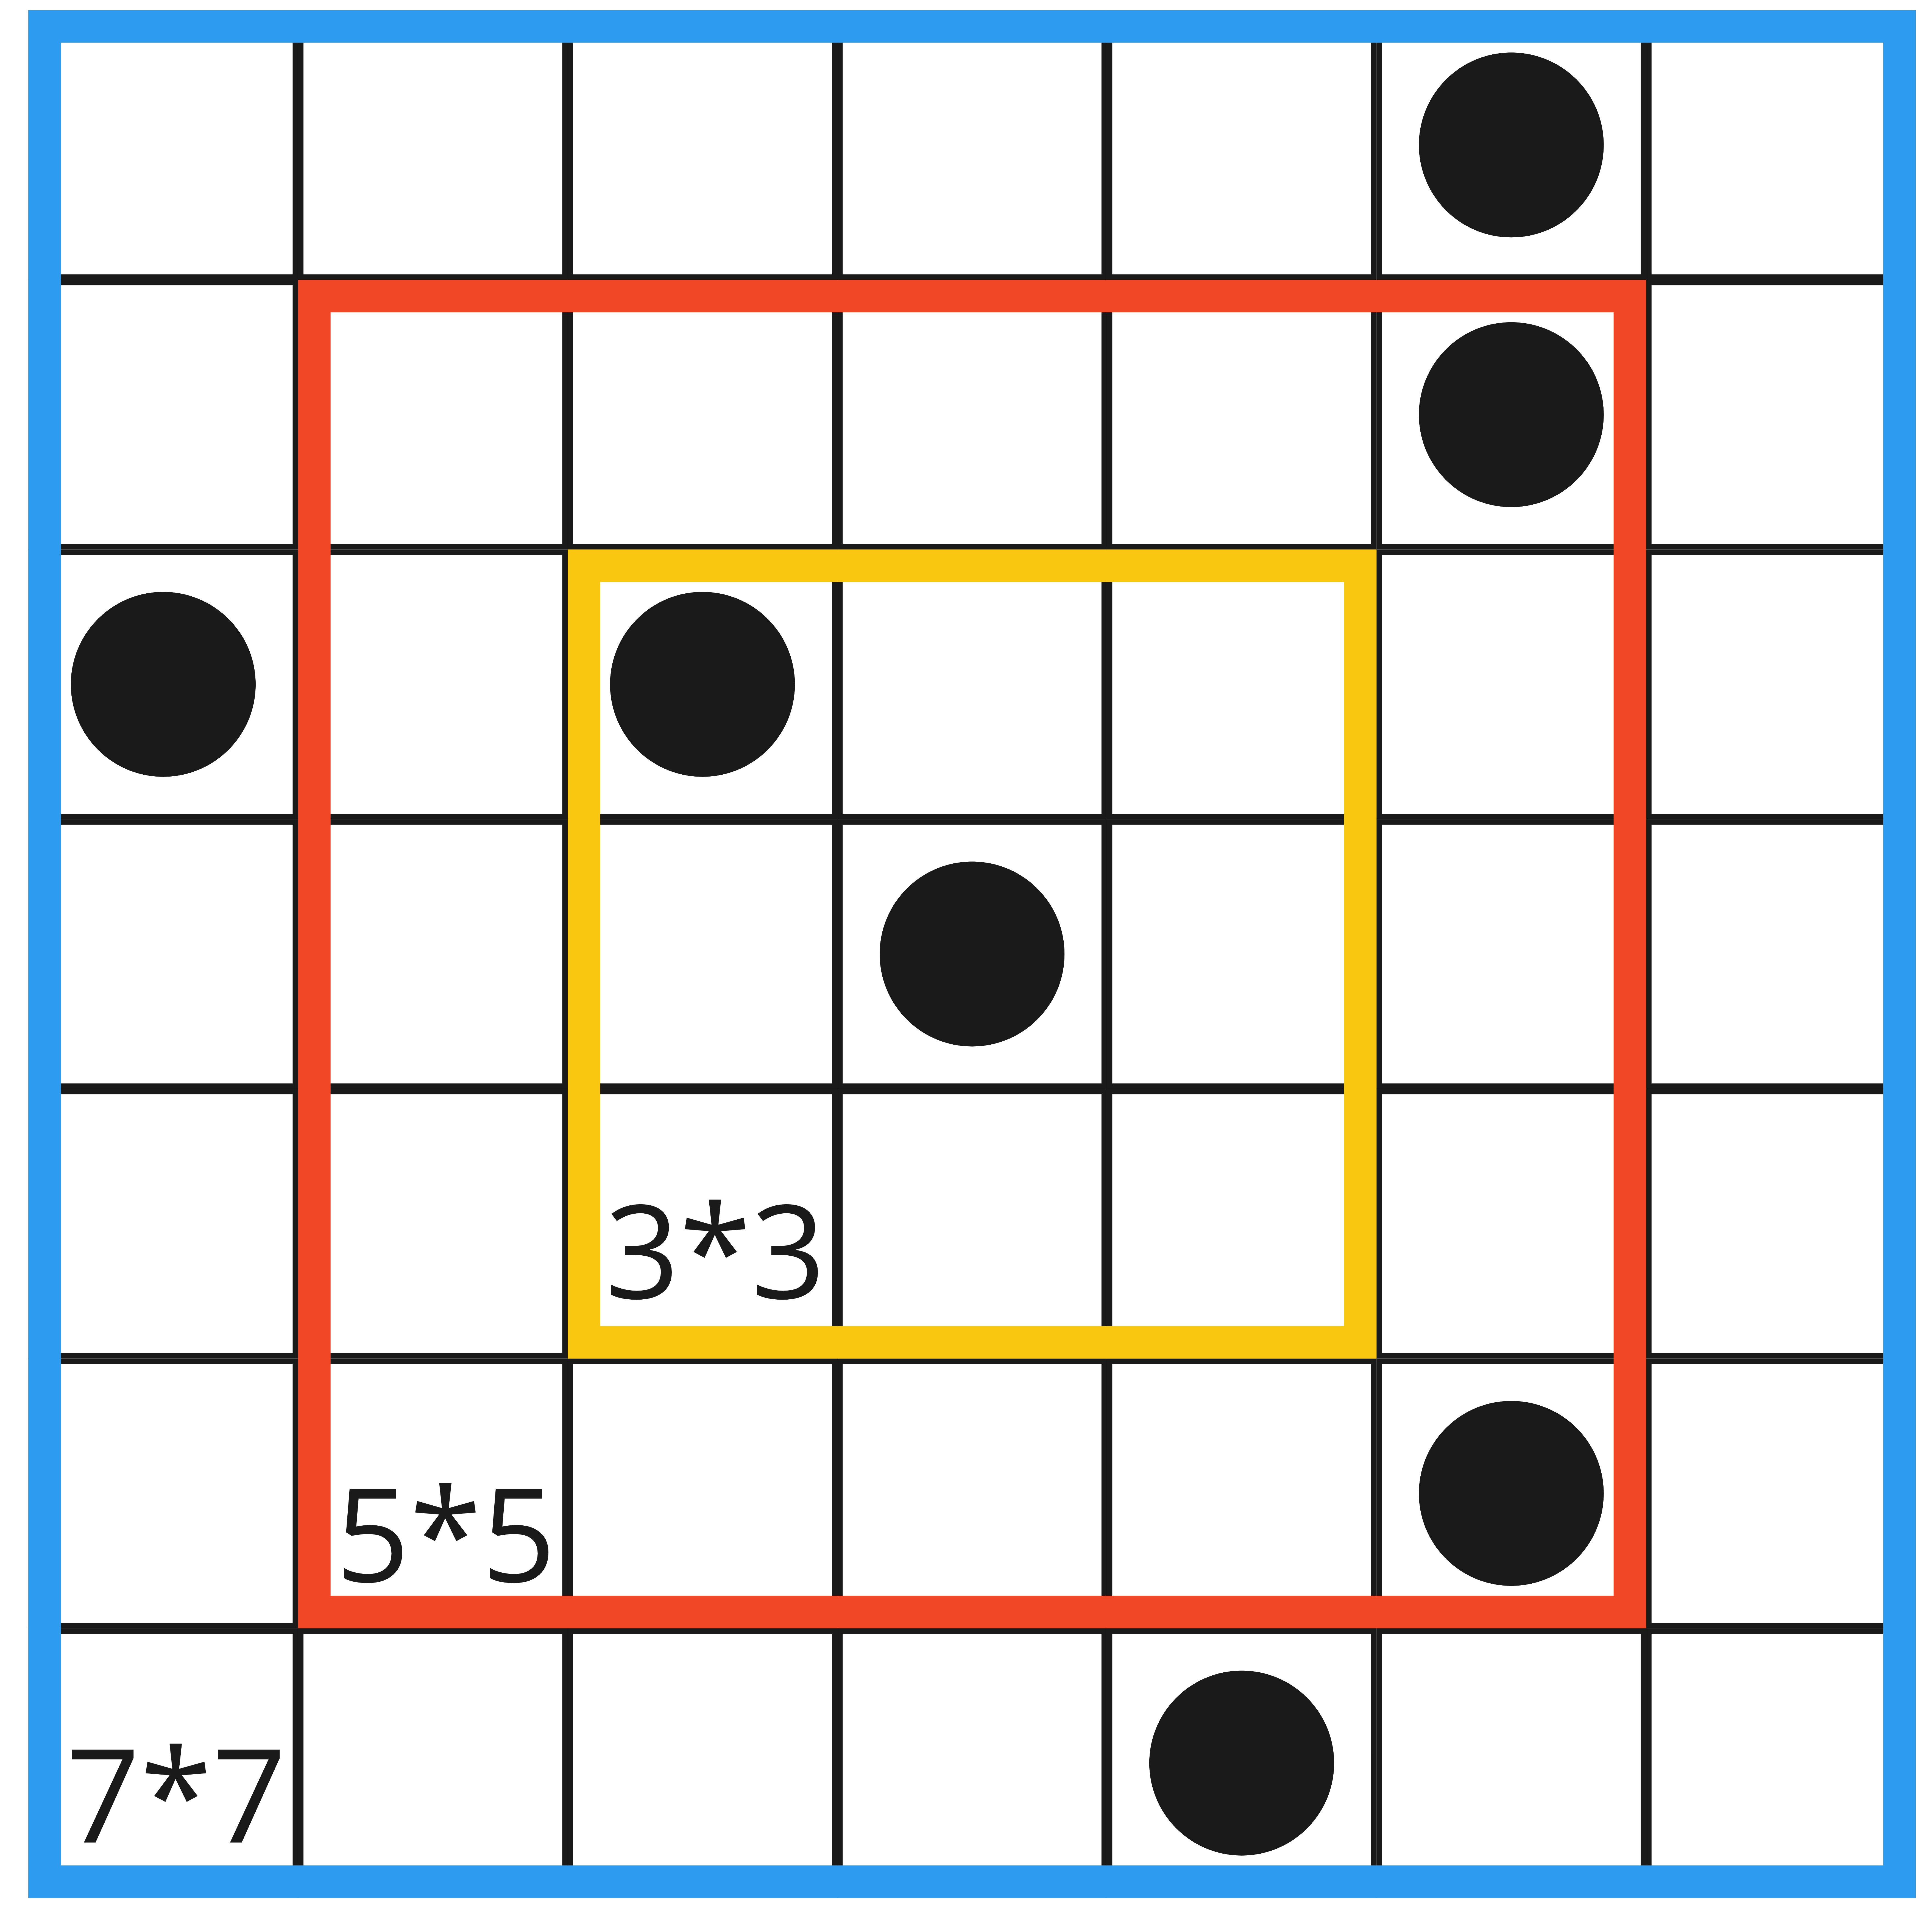
\includegraphics[width=3in]{img/Neighbor/intro.jpg}
\caption{Fractal Dimension vs. Neighboring Ranges
\label{neiintro}}
\end{figure}

Neighboring range, $l_{\rm neigh}$, refers to the range that determines whether a random walker is near a cluster. A $3\times3$ neighboring range would detect whether there is a particle that belongs to the cluster is within the $x$ range of $x-1$ to $x+1$ and $y$ range of $y-1$ and $y + 1$ (See Fig.~\ref{neiintro}).

\begin{figure}[h]
     \centering
     \begin{subfigure}[h]{0.23\textwidth}
         \centering
         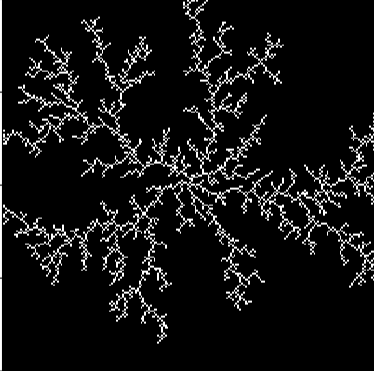
\includegraphics[width=\textwidth]{img/Neighbor/3.png}
         \caption{neighbor range=3}
         \label{nr3}
     \end{subfigure}
     \hfill
     \begin{subfigure}[h]{0.23\textwidth}
         \centering
         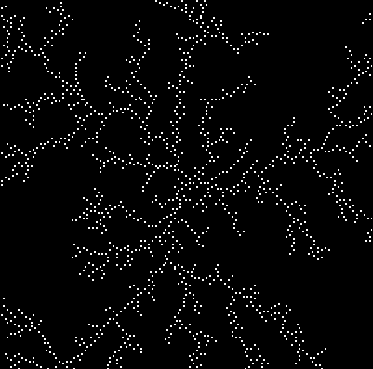
\includegraphics[width=\textwidth]{img/Neighbor/5.png}
         \caption{neighbor range=5}
         \label{nr5}
     \end{subfigure}
     \hfill
     \begin{subfigure}[h]{0.23\textwidth}
         \centering
         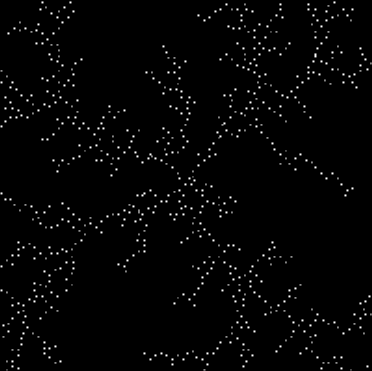
\includegraphics[width=\textwidth]{img/Neighbor/7.png}
         \caption{neighbor range=7}
         \label{nr7}
     \end{subfigure}
     \hfill
     \begin{subfigure}[h]{0.23\textwidth}
         \centering
         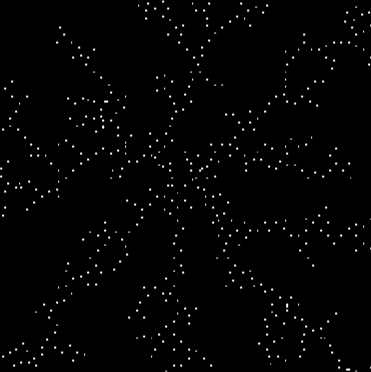
\includegraphics[width=\textwidth]{img/Neighbor/9.png}
         \caption{neighbor range=9}
         \label{nr9}
     \end{subfigure}
        \caption{Clusters with Neighboring Range ($N=3000$)}
        \label{nrs}
\end{figure}

The higher the neighboring range is the distance between two points in the cluster would be farther. As indicated from the graphs above from left to right (See Fig.~\ref{nrs}), we have neighboring ranges from $3 \times 3$ to $9 \times 9$. When the neighboring range is small, the particles in the cluster are prone to be closer to each other, while when we increase the neighboring range of the particles in the cluster, the gap between particles increases. At the same time, given a particular range, the density of the cluster would decrease as well. One way to verify this is that we can see from the difference between the cluster with neighboring range $9 \times 9$ and the cluster with neighboring range $3 \times 3$, the image with a higher neighboring range is dimmer than the image with a lower neighboring range. This is a result of more dark points within the cluster, which is a direct result of the increased distance between particles. 

\begin{figure}[h]
\centering
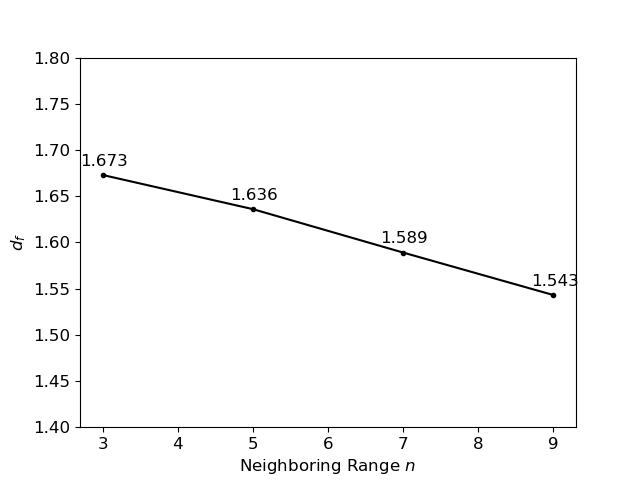
\includegraphics[width=4.0in]{img/Neighbor/dfNeighbor.png}
\caption{Fractal Dimension vs. Neighboring Ranges
\label{dfnr}}
\end{figure}

We also measure the fractal dimension of the cluster with different neighboring ranges. As we increased n from 3 to 9,  we could observe a negative linear-like relationship between the decreases of fractal dimension and increases of neighboring ranges (See Fig.~\ref{dfnr}). The slope of this decrease has a mean of around  -0.042. At the neighboring range equaling to $3 \times 3$ (See Fig.~\ref{neiintro}), when we checking the nearby location of the random walker, the actual number of locations we check is 8 that is close to the default settings with 4 locations to check. As a consequence, the fractal dimension is also close to the actual fractal dimension of the DLA model in default settings with value of 1.71. On the other hand, at the neighboring range equaling to $9 \times 9$, due to the spareness of the cluster, the fractal dimension of such a cluster is relatively much lower. 

\subsection{Off-Lattice Result}
\subsubsection{Alpha}

The variation of $\alpha$ is only applicable in off-lattice simulation. According to Eq.~\ref{off}, $\alpha$ refers to the step size of each random walker step size. As shown in Fig.~\ref{alpha}, the higher $\alpha$, the structure of cluster is more constricted. For a small $\alpha$ is low (for example, $\alpha = 2$), we observe a pattern where every branch of cluster is more spread out than for larger $\alpha$ (such as $\alpha = 4$). This is a result of the overlapping between any of two particles within the cluster (See Fig.~\ref{ol}). Since off-lattice simulation allows for overlapping between particles, the higher the $\alpha$, the larger likelihood of overlapping. If two particles overlap, the total area of the two particles is smaller.

\begin{figure}[h]
     \centering
     \begin{subfigure}[h]{0.23\textwidth}
         \centering
         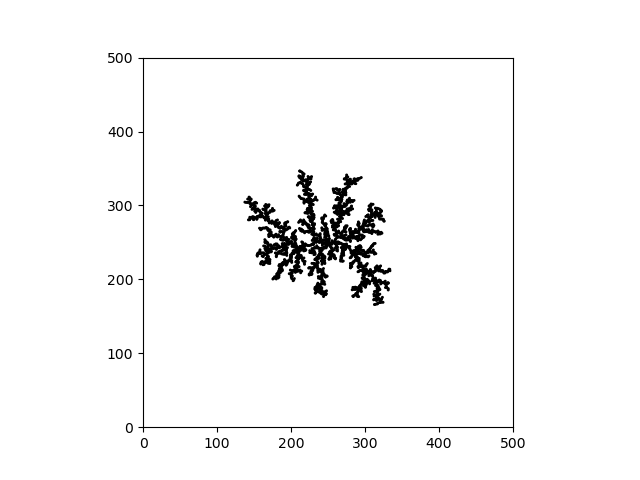
\includegraphics[width=\textwidth]{img/alpha/2.png}
         \caption{$\alpha = 2$}
         \label{al3}
     \end{subfigure}
     \hfill
     \begin{subfigure}[h]{0.23\textwidth}
         \centering
         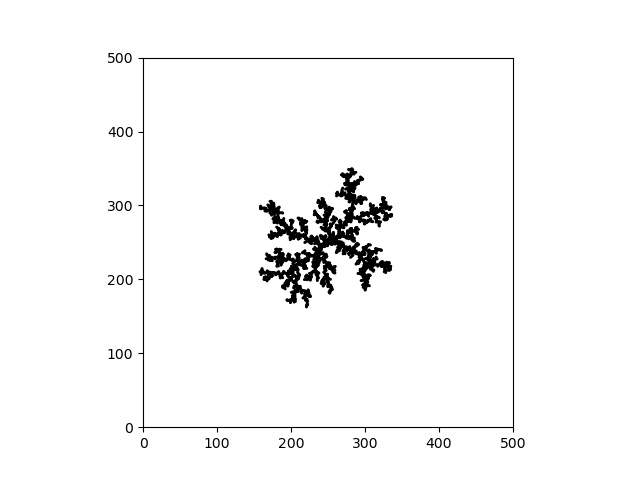
\includegraphics[width=\textwidth]{img/alpha/3.png}
         \caption{$\alpha = 3$}
         \label{al5}
     \end{subfigure}
     \hfill
     \begin{subfigure}[h]{0.23\textwidth}
         \centering
         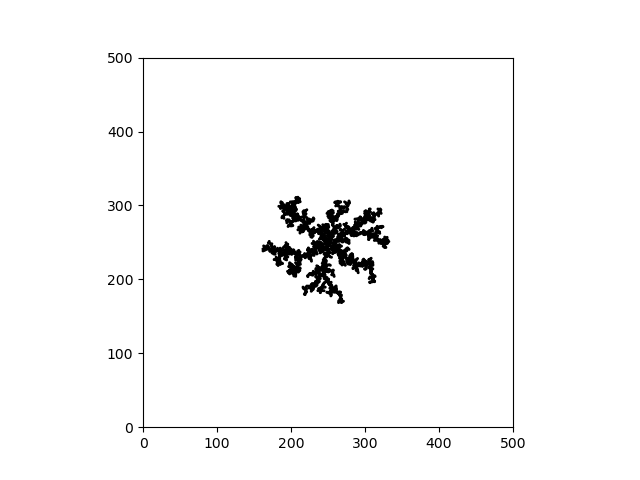
\includegraphics[width=\textwidth]{img/alpha/4.png}
         \caption{$\alpha = 4$}
         \label{al7}
     \end{subfigure}
     \hfill
     \begin{subfigure}[h]{0.23\textwidth}
         \centering
         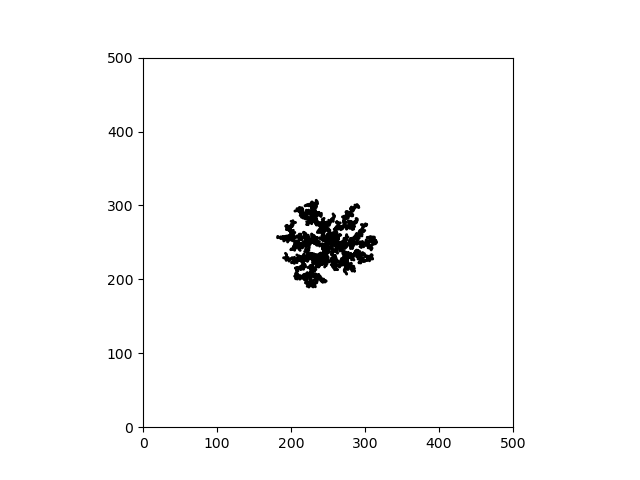
\includegraphics[width=\textwidth]{img/alpha/5.png}
         \caption{$\alpha = 5$}
         \label{al9}
     \end{subfigure}
        \caption{Clusters with Random Walk Step Size $\alpha$}
        \label{alpha}
\end{figure}

\begin{figure}[h]
     \centering
     \begin{subfigure}[h]{0.45\textwidth}
         \centering
        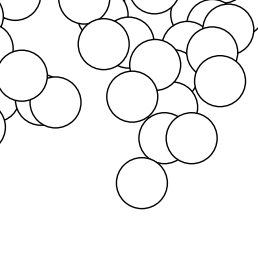
\includegraphics[width=2.0in]{img/alpha/ol.png}
        \caption{Overlapping in Off-lattice Simulation
        \label{ol}}
     \end{subfigure}
     \hfill
     \begin{subfigure}[h]{0.45\textwidth}
         \centering
        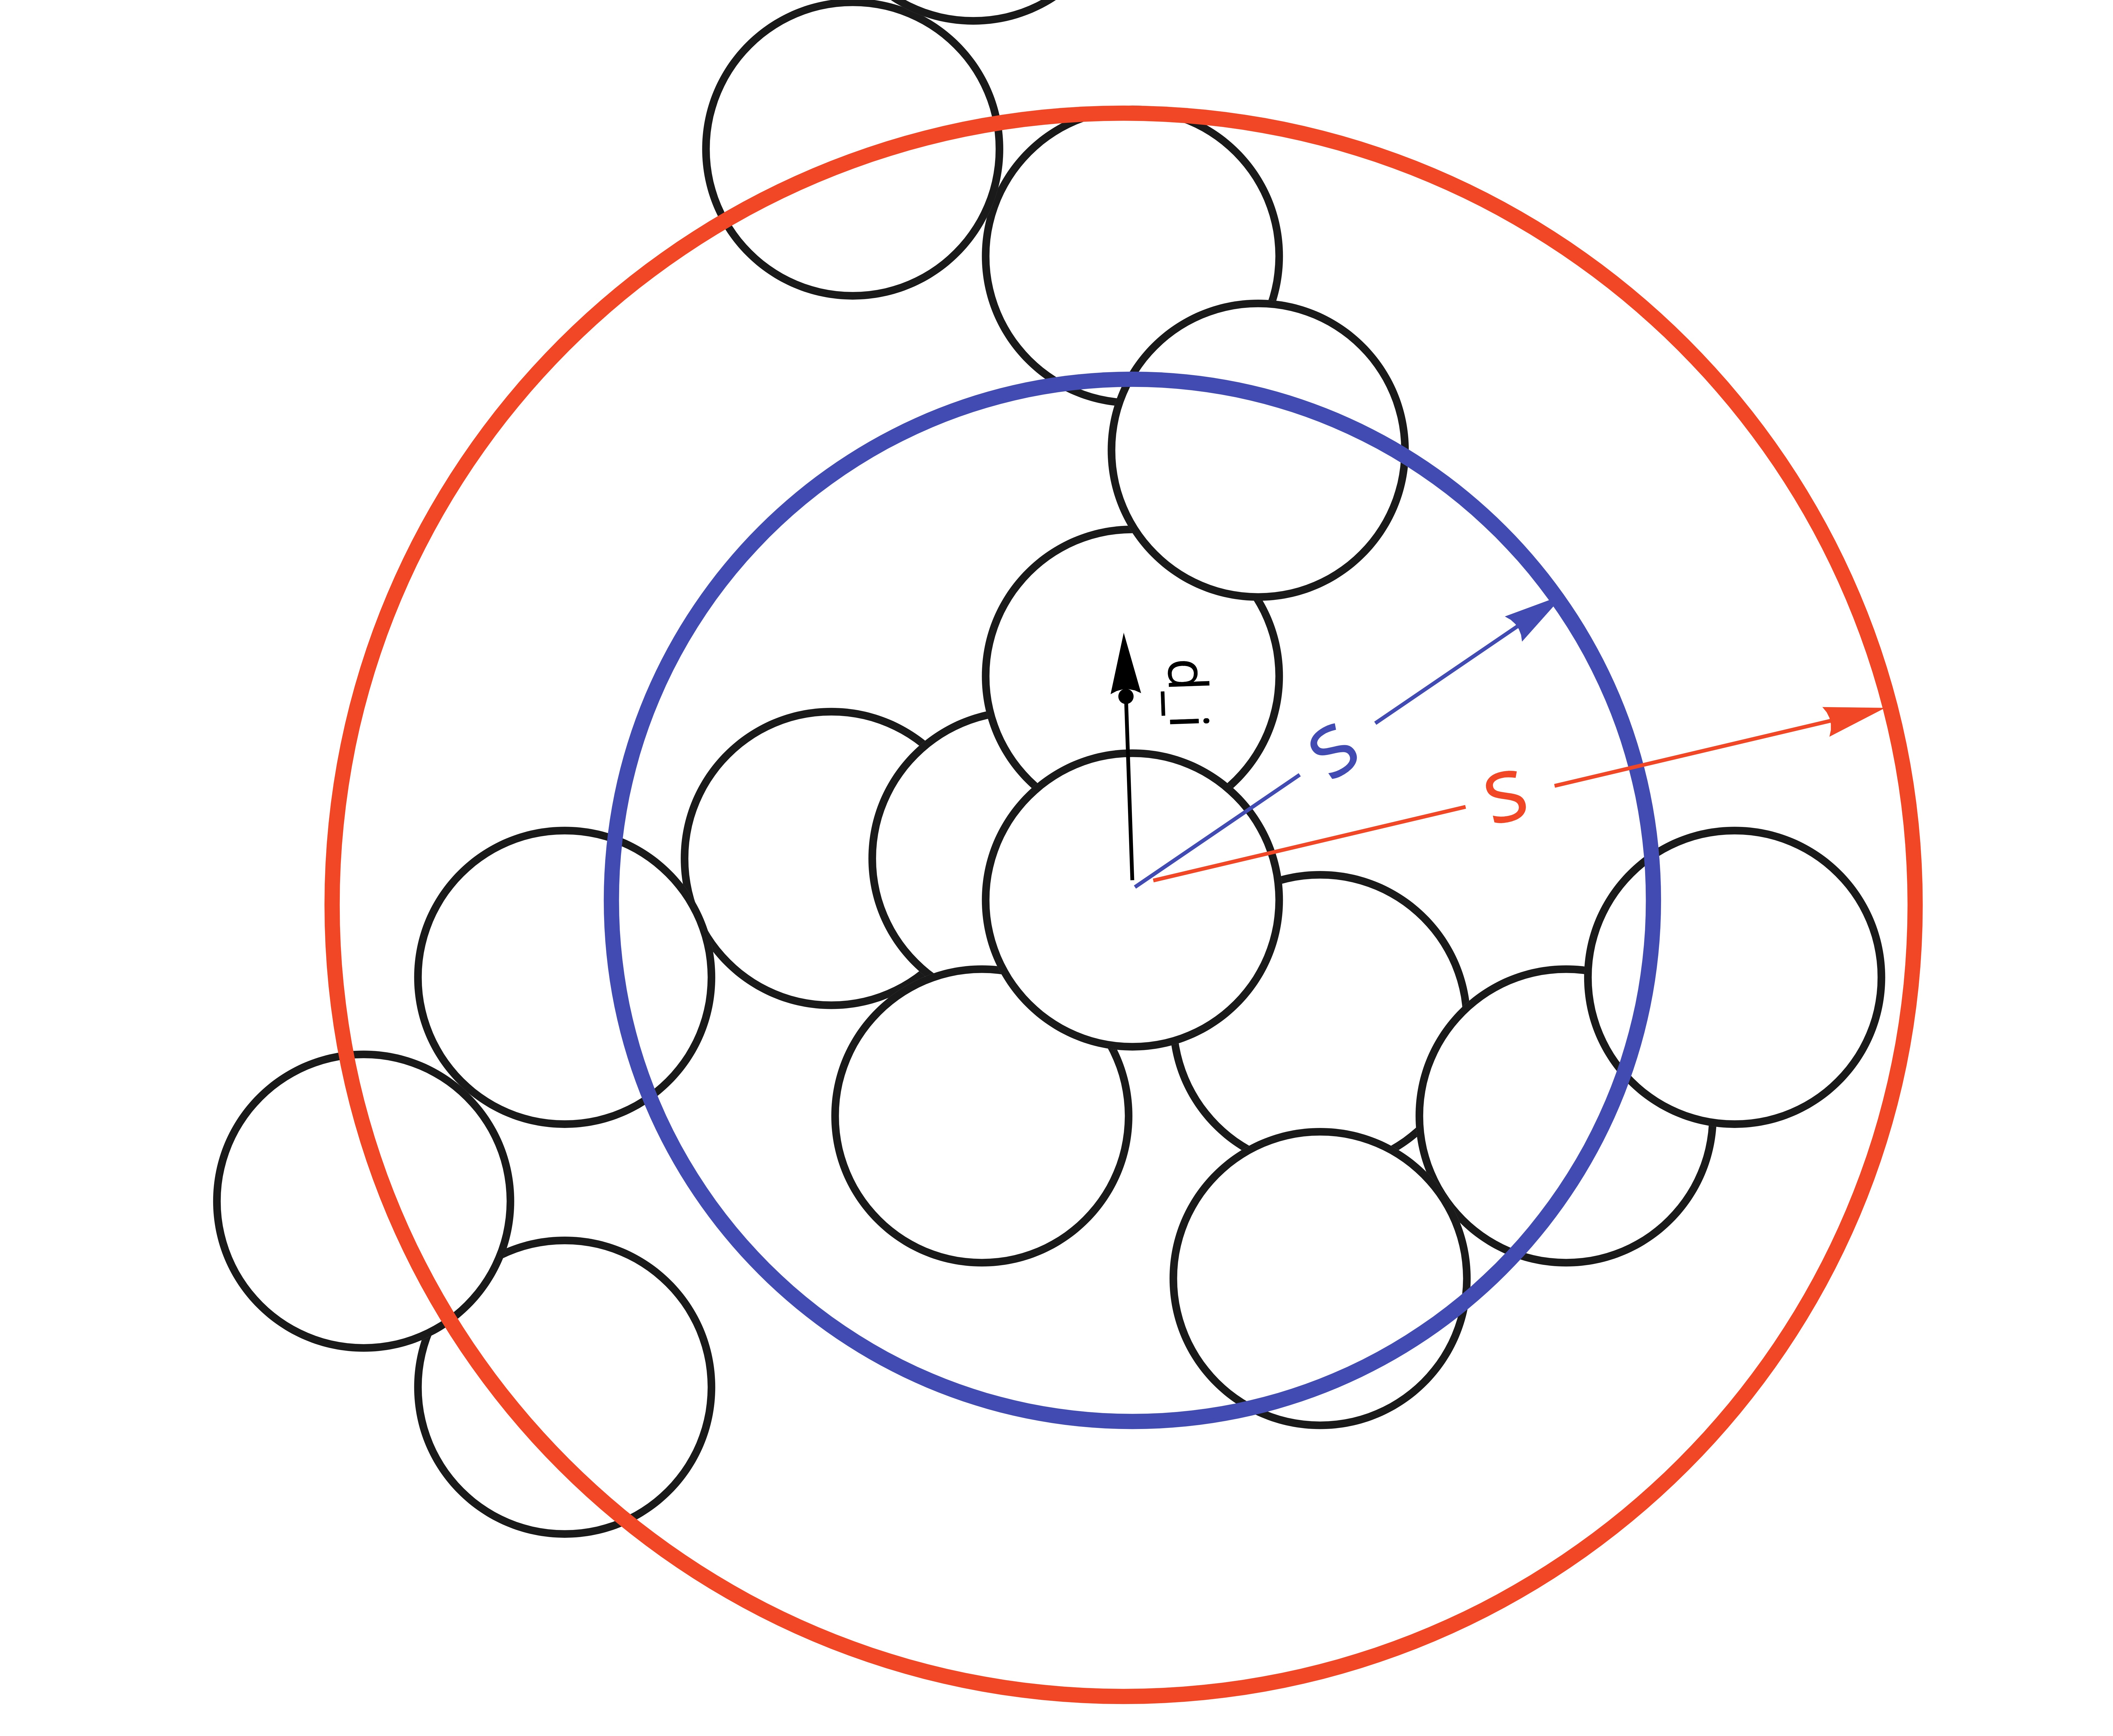
\includegraphics[width=2.0in]{img/sr.jpg}
        \caption{Calculation of Fractal Dimension
        \label{dfr}}
     \end{subfigure}
\end{figure}


here we determine the effect of $\alpha$ on the fractal dimension. Unlike calculating fractal dimension of an on-lattice pattern, we use a circle with radius $s$ instead of using a box to measure the fractal dimension of off-lattice simulation  (see Fig.~\ref{dfr}). To calculate the number of particles within the circle, for each particle $i$ belonging to cluster, we calculate the distance $d_i$ between the position of particle, $(x_i,y_i)$, and the position of center, $(x_c,y_c)$, where
\[
d_i = \sqrt{(x_i-x_c)^2+(y_i-y_c)^2}
\]
we count the number of particles with $d_i$ less than the radius of circle, $d_i<s$.

\begin{figure}[h]
\centering
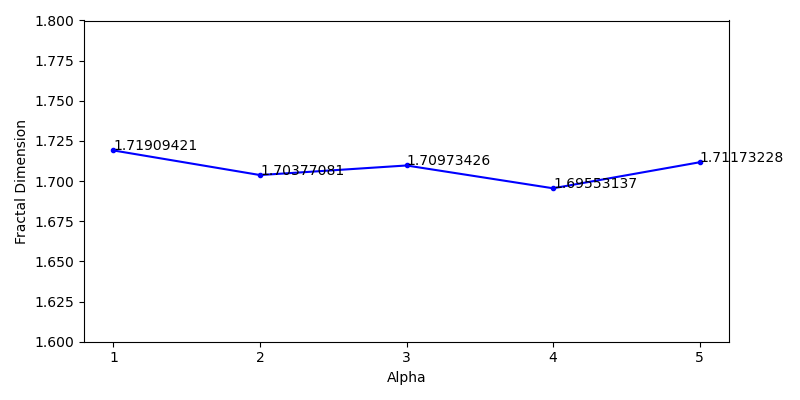
\includegraphics[width=5.0in]{img/alpha/dfalpha.png}
\caption{Fractal Dimension vs. Alpha (Cluster Size 3000)
\label{dfa}}
\end{figure}

Similar to the on-lattice case, we obtain $d_f$ as the slope of a linear fit to $\log(N)$ as a function of $\log(s)$. The resulting $d_f$ as function of $alpha$ is shown in Fig.~\ref{dfa}. The measured fractal dimension of all $\alpha$ is close to each other. Even if there are some fluctuations among these values. The standard deviation of these values is around 0.008, which is quite small. Thus, we can conclude that although visually the cluster is more constricted when we have a high value of alpha, the fractal dimension is independent of $\alpha$.

\section{Conclusion}

In this paper, we examine some characteristics within DLA model by calculating and comparing the fractal dimension under various conditions. We determine $d_f$ as function of the number of particles in the cluster, and find that the cluster size at the end of simulation with 3000 particles is in the leveled off region, where the fractal dimension is close to the expected value of 1.71. Therefore, we set all the following simulations to 3000 particles and we found a negative linear-like relationship between the decreases of fractal dimension, which is lower than the accepted value 1.71, and increases of neighboring ranges. We also found that the lower the stickiness, the higher the fractal dimension, which is higher than the accepted value 1.71. however, not every changes in parameters of simulation would cause the change in fractal dimension. For example, when we change the $\alpha$ in off-lattice simulation, there is not fundamental changes in measured fractal dimensions. Thus, we can conclude that the fractal dimension depends on stickiness and neighboring range in on-lattice simulations but is independent of $\alpha$ in off-lattice simulations. The future work of DLA simulation can focus on examine other parameters within the simulation, such as changing the radius of every particle in off-lattice simulation and changing the movement of random walker in on-lattice simulation. 

\bibliography{myRefs}  

\end{document} 
